%% ==============================
\chapter{Methoden der Dimensionsreduktion}
\label{ch:MethodenDerDimRed}
%% ==============================

Nachdem nun die Motivation und Idee hinter der Dimensionsreduktion in \chapref{ch:Enleitung} und
die mathematische Formulierung in \chapref{ch:Dimensionsreduktion} allgemein angeschaut wurde,
werden nun einige konkrete Methoden der Dimensionsreduktion vorgestellt.

In jüngster Zeit haben vor allem verschiedenste Varianten von neuronale Netzen einen hohen Grad an
Aufmerksamkeit durch bemerkenswerte Errungenschaften in Gebieten der automatischen Spracherkennung
oder \textit{Computer Vision} erlangt. Fraglich ist, ob diese neuen Algorithmen auch auf dem
Bereich der Dimensionsreduktion einen entscheidenden Fortschritt gemacht haben. Deshalb werden die
Algorithmen in dieser Arbeit in \textit{statistischen} und \textit{Machine Learning} Methoden
unterteilt, um diese später in \chapref{ch:Vergleich} gegenüberstellen zu können. Statistische
Methoden haben eine solide theoretische Fundierung und sind meist etablierte Algorithmen auf einem
jeweiligen Gebiet, wie das zum Beispiel mit der Hauptkomponentenanalyse
(\subsecref{ch:MethodenDerDimRed:statistisch:PCA}) der Fall ist. Machine Learning Methoden hingegen
haben lediglich das Ziel, von Trainingsdaten auf neue, das heißt ungesehene (Test-)Daten zu
generalisieren. Neuronale Netze sind hierfür ein Paradebeispiel und werden deshalb in
\secref{ch:MethodenDerDimRed:modern} eingehend behandelt. Allerdings ist hier aus jeder Kategorie
nur eine kleine repräsentative Auswahl getroffen worden. Weitere wichtige Algorithmen, die hier
nicht vorgestellt werden können sind beispielsweise \dots \todo{Aufzählung der Algorithmen die
	nicht betrachtet werden hier oder in der Einleitung?}.

\section{Statistische Methoden}
\label{ch:MethodenDerDimRed:statistisch}

Zu den statistischen Methoden, die in dieser Arbeit vorgestellt werden, gehören die
\newterm{Hauptkomponentenanalyse} (PCA) in \subsecref{ch:MethodenDerDimRed:statistisch:PCA} sowie
die nichtlineare Erweiterung der Hauptkomponentenanalyse, die Kernel PCA
(\subsecref{ch:MethodenDerDimRed:statistisch:kPCA}). Außerdem wird die Multidimensionale Skalierung
(MDS) in \subsecref{ch:MethodenDerDimRed:statistisch:MDS} als Vertreter der statistischen Methoden
genauer behandelt.

%% ==============================
\subsection{Principal Component Analysis}
\label{ch:MethodenDerDimRed:statistisch:PCA}
\nomenclature[Z]{PCA}{Principal Component Analysis}

Principal Component Analysis ist \textit{die} Methode der Dimensionsreduktion und wurde erstmals
von \textcite{Pearson.1901} und \textcite{Hotelling.1933} entwickelt. Trotz des mittlerweile
relativ hohen Alters ist die Hauptkomponentenanalyse immer noch aufgrund der simplen Anwendbarkeit
oft die erste Wahl einer Dimensionsreduktionsmethode. Im Folgenden möchte ich kurz auf die zentrale
Idee und Motivation (\ref{ch:MethodenDerDimRed:statistisch:PCA:Grundidee}) der
Hauptkomponentenanalyse, sowie die mathematische Herleitung der sogenannten
\newterm{Hauptkomponenten} (Unterabschnitte \ref{ch:MethodenDerDimRed:statistisch:PCA:Definition}
und \ref{ch:MethodenDerDimRed:statistisch:PCA:HerleitungPC}) eingehen.

\subsubsection{Grundidee}
\label{ch:MethodenDerDimRed:statistisch:PCA:Grundidee}
Die zentrale Idee der Hauptkomponentenanalyse ist die Transformation des Koordinatensystems in einer möglichst \textit{verlustfreien} Art und Weise. Verlustfrei bedeutet im Kontext der Hauptkomponentenanalyse, dass möglichst viel Variation in den Daten erhalten bleiben soll \parencite[vgl.][1]{Jolliffe.2002}. Möchte man dann die Dimension von $D$ auf die intrinsische
Dimension $d$ reduzieren, so wählt man einfach die \textit{ersten} $d$ Hauptkomponenten.\rewrite{Zu
	ungenau, und hier gleich das Ergebnis zu erwähnen ist auch nicht so hilfreich für die Grundidee}
Was diese Hauptkomponenten sind und wie man sie herleitet, wird im Folgenden genauer betrachtet.

\subsubsection{Definition der Hauptkomponenten}
\label{ch:MethodenDerDimRed:statistisch:PCA:Definition}
Als Ausgangsbasis wird ein $D$-dimensionalen Zufallsvektor $\rvect{x} = \tr{(\rv{x}_1, \ldots, \rv{x}_D)}$ mit $\Exp[\rvect{x}] = \vect{0}$ angenommen und das Ziel ist es, eine $k$-dimensionale Repräsentation $\rvect{y} = \tr{(\rv{y_1},\ldots,\rv{y}_k)}$ zu erhalten. Idealerweise setzt man $k$ auf die intrinsische Dimension $d$ von $\rvect{x}$, hier soll jedoch nur der Fokus auf die allgemeine Dimensionsreduktion gelegt werden. Wir drücken also $\rvect{y}$ als eine Linearkombination des ursprünglichen hochdimensionalen Vektors $\rvect{x}$ wie folgt aus:
\begin{equation}
	\rv{y}_i = \tr{\vect{a}_i} \rvect{x} = a_{i1} \rv{x}_1 + \cdots + a_{iD} \rv{x}_D
	\quad i = 1,\ldots,k
\end{equation}
wobei $\vect{a}_i$ die \newterm{Koeffizienten} (auch: Ladungen) der $i$-ten Hauptkomponente sind \parencite[vgl.][2]{Jolliffe.2002}. Die Anzahl $k$ der Hauptkomponenten bestimmt den Grad der
Dimensionsreduktion, kann jedoch beliebig zwischen $1 \leq k \leq D$ gewählt werden.\footnote{Der
	Grenzfall $k = D$ wird oft für eine Anonymisierung des Datensatzes mit personenbezogenen Daten
	verwendet. Beispielsweise kann so bei Finanztransaktionen der Datensatz mithilfe von PCA
	vorverarbeitet (\textit{Preprocessing}) und erst dann veröffentlicht werden.}

\subsubsection{Herleitung der Hauptkomponenten}
\label{ch:MethodenDerDimRed:statistisch:PCA:HerleitungPC}
Betrachtet wird nun zunächst lediglich die \textit{erste} Hauptkomponente $\tr{\vect{a}_1} \rvect{x}$ und erinnern uns daran, dass wir wie in \subsecref{ch:MethodenDerDimRed:statistisch:PCA:Grundidee} erwähnt möglichst viel Variation von $\rvect{x}$ erhalten möchten. Daher wird die erste Hauptkomponente so gewählt, dass die Varianz maximal wird:
\begin{equation}
	\label{eq:PCA-Optimierungsproblem}
	\max_{\vect{a}_1} \Var \left( \tr{\vect{a}_1} \rvect{x} \right) = \max_{\vect{a}_1} \tr{\vect{a}_1} \mat{\Sigma} \vect{a}_1
\end{equation}
wobei $\mat{\Sigma}$ die Kovarianzmatrix von $\rvect{x}$ ist. Dieses Maximierungsproblem ist jedoch nach oben unbeschränkt, weshalb man zusätzlich die Bedingung
\begin{equation}
	\norm{ \vect{a}_1 }^2 = \tr{\vect{a}_1} \vect{a}_1 = 1
\end{equation}
zum nun \textit{restringierten} Maximierungsproblem hinzufügt, welches mithilfe des Lagrange-Ansatzes gelöst werden kann. Diese Bedingung führt dazu, dass wir eine orthogonale Transformation\unsure{Zitat hinzufügen oder mehr dazu sagen, ein satz reicht nicht} erhalten. Wie sich heraustellt, ist dieses Maximierungsproblem ein Eigenwertproblem und kann somit effizient gelöst werden \parencite[vgl.][4 -- 6]{Jolliffe.2002}\unsure{Vlt hier die Lagrange Gleichung aufstellen und selber
	lösen, um zu sehen, dass man bei einem Eigenwertproblem landet}. Man erhält somit die Koeffizienten
der ersten Hauptkomponente $\vect{a}_1$, welche ein Eigenvektor von $\mat{\Sigma}$ mit zugehörigem
Eigenwert
\begin{equation}
	\lambda_1 = \Var(\tr{\vect{a}_1} \rvect{x})
\end{equation}
sind. Man beachte, dass dies gleichzeitig die Zielfunktion unseres Optimierungsproblems (\eqref{eq:PCA-Optimierungsproblem}) ist. Das bedeutet, dass die Koeffizienten der ersten Hauptkomponente dem Eigenvektor mit dem größten zugehörigen Eigenwert entspricht.

Um nun die zweite Hauptkomponente zu erhalten, wird wieder die Varianz mit der
Einheitsvektor-Nebenbedingung $\norm{\vect{a}_2}$ = 1 maximiert. Zusätzlich muss jedoch gelten,
dass die zweite Hauptkomponente zur Ersten \textit{unkorreliert}\unsure{wieso muss das gelten? Ein
	satz dazu wäre gut} ist \parencite[5]{Jolliffe.2002}, das heißt
\begin{equation}
	\Cov(\tr{\vect{a}_1}\rvect{x}, \tr{\vect{a}_2}\rvect{x}) = 0
\end{equation}
Auch dieses Optimierungsproblem ist ein Eigenwertproblem und man erhält, dass die Koeffizienten $\vect{a}_2$ der zweiten Hauptkomponente der Eigenvektor mit dem zweitgrößten Eigenwert von $\mat{\Sigma}$ ist.
Generell lässt sich zeigen, dass die Koeffizienten der $i$-ten Hauptkomponente dem Eigenvektor mit $i$-ten nach der Größe geordneten Eigenwert entspricht \parencite[6]{Jolliffe.2002}. Aus diesem Grund lassen sich die Hauptkomponenten kompakt durch
\begin{equation}
	\rvect{y} = \tr{\mat{A}} \rvect{x}
\end{equation}
ausdrücken, wobei $\mat{A} = [\vect{a}_1,\ldots,\vect{a}_k] \in \real^{D \times k}$ die Matrix der Eigenvektoren als Spaltenvektoren ist und wieder $1 \leq k \leq D$ gilt.

\subsubsection{Erweiterungen}
\label{ch:MethodenDerDimRed:statistisch:PCA:Erweiterungen}
Trotz der großen Beliebtheit der Hauptkomponentenanalyse hat diese Methode natürlich auch ihre Nachteile, weswegen zahlreiche Erweiterungen wie zum Beispiel \ldots\addref entwickelt wurden.
Ein Schwachpunkt von PCA ist, dass die orthogonale Transformation auf die Eigenvektorbasis der Kovarianzmatrix inhärent linear ist. Die Hauptkomponentenanalyse ist also in dieser klassischen Form nicht in der Lage, eine nichtlineare Mannigfaltigkeit in den Daten zu erkennen. Deswegen wurde unter anderem eine Generalisierung von PCA von \textcite{Scholkopf.1997} entwickelt, die sogenannte \newterm{Kernel Principal Component Analysis} (kPCA). Diese Methode wird in \subsecref{ch:MethodenDerDimRed:statistisch:kPCA} genauer behandelt.

%% ==============================
\subsection{Kernel Principal Component Analysis}
\label{ch:MethodenDerDimRed:statistisch:kPCA}
\nomenclature[Z]{kPCA}{Kernel Principal Component Analysis}
Wie soeben erwähnt ist die Kernel Principal Components Analysis insofern eine Generalisierung der klassischen Hauptkomponentenanalyse, dass auch nichtlineare Zusammenhänge erkannt werden können.
Um das zu erreichen, wird sich am sogenannten \newterm{Kernel Trick} bedient, der schon erfolgreich auf \textit{Support Vector Machines} \parencite{Boser.1992} angewandt wurde. Dazu gehen wir wieder in
\subsecref{ch:MethodenDerDimRed:statistisch:kPCA:Grundidee} auf die Grundidee dieser Methode ein
und befassen uns dann in \subsecref{ch:MethodenDerDimRed:statistisch:kPCA:Vorgehensweise} kurz mit
der konkreten Vorgehensweise bei der Kernel PCA.

\subsubsection{Grundidee}
\label{ch:MethodenDerDimRed:statistisch:kPCA:Grundidee}

Die Grundidee der Kernel PCA ist es, die Daten mithilfe einer Funktion $\bm{\phi}$ in einen
Vektorraum $\mathcal{H}$ abzubilden, der nichtlinear mit dem Ursprungsraum $\mathcal{X}$ verbunden
ist. Der Raum $\mathcal{H}$ wird in diesem Kontext auch Merkmalsraum (engl. \textit{feature space})
genannt und kann potentiell sehr hochdimensional sein. Nach der Transformation wird also die
traditionelle Hauptkomponentenanalyse durchgeführt, um damit die niedrigdimensionale Repräsentation
$\rvect{y}$ zu erhalten. Dies erscheint auf den ersten Blick kontraintuitiv, da durch den
\enquote{Umweg} über die Abbildung $\bm{\phi}$ die Dimension zuerst erhöht wird. Motiviert wird es
dadurch, dass die Daten in $\mathcal{X}$ einen \textit{nichtlinearen} Zusammenhang aufweisen
können, während in $\mathcal{H}$ der Zusammenhang linear und damit für lineare Algorithmen wie die
Hauptkomponentenanalyse erkennbar ist \parencite[vgl.][26]{ShaweTaylor.2011}.

Der entscheidende Punkt ist jedoch, dass man die Abbildung $\bm{\phi}$ nicht explizit berechnet,
sondern mithilfe einer Kernel-Funktion $\kappa: \mathcal{X} \times \mathcal{X} \rightarrow \real$
implizit gegeben hat \parencites[586 -- 588]{Bishop.2006}[583]{Scholkopf.1997}. Der Kernel Trick ist immer dann anwendbar,
wenn der Algorithmus so formuliert werden kann, dass $\bm{\phi}$ ausschließlich als Skalarprodukt
vorkommt. Im Folgenden wird die Vorgehensweise bei der Kernel PCA kurz erläutert, allerdings wird
für eine eingehendere Behandlung des Kernel Tricks und anderer Kernel-Methoden auf
\textcite{ShaweTaylor.2011} verwiesen.

\subsubsection{Der Kernel}
\label{ch:MethodenDerDimRed:statistisch:kPCA:KernelFunktion}

Ein Kernel $\kappa$ ist definiert als das Skalarprodukt im Merkmalsraum \parencite[34]{ShaweTaylor.2011}
\begin{equation}
	\label{eq:kPCA:KernelFunction}
	\kappa(\vect{x}_i, \vect{x}_j) = \tr{\bm{\phi}(\vect{x}_i)} \bm{\phi}(\vect{x}_j)
\end{equation}
und ist damit intuitiv gesehen ein \enquote{Orakel} für die Ähnlichkeit der Daten im Merkmalsraum, weil dies ohne Kenntnis der Koordinaten berechnet werden kann \parencite[71]{ShaweTaylor.2011}. Wie bereits in
\subsecref{ch:MethodenDerDimRed:statistisch:kPCA:Grundidee} erwähnt, muss die
Hauptkomponentenanalyse nun in eine Form gebracht werden, in der nur Skalarprodukte von
$\bm{\phi}(\rvect{x})$ vorkommen. Diese Skalarprodukte können dann gemäß
\eqref{eq:kPCA:KernelFunction} durch die Kernel-Funktion ersetzt werden.

In der Praxis häufig anzutreffen sind der Gauß-Kernel ...

\unsure{Kernel-Matrix hier definieren?}

\subsubsection{Vorgehensweise}
\label{ch:MethodenDerDimRed:statistisch:kPCA:Vorgehensweise}
Die Kovarianzmatrix $\mat{C}$ der (zentrierten) Daten im Merkmalsraum ist definiert als
\begin{equation}
	\mat{C} = \frac{1}{n} \tr{\bm{\phi}(\mat{X})} \bm{\phi}(\mat{X}) \, ,
\end{equation}
wobei $\bm{\phi}$ hier elementweise angewandt wird. Um nun die Hauptkomponentenanalyse durchführen zu können, müssten die Eigenvektoren dieser Matrix bestimmt werden. Dies ist jedoch nicht möglich, da die Abbildung $\bm{\phi}$ unbekannt ist. Wie sich herausstellt ist diese Matrix aber sehr ähnlich zur sogenannten \textit{Kernel Matrix} $\mat{K}$, welche über den Kernel $\kappa$ als
\begin{align}
	\mat{K} & = \left( \kappa(\vect{x}_i, \vect{x}_j) \right)_{i,j = 1,\ldots,n} \label{eq:kPCA:KernelMatrix_A} \\
	        & = \bm{\phi}(\mat{X}) \tr{\bm{\phi}(\mat{X})} \label{eq:kPCA:KernelMatrix_B}
\end{align}
definiert ist \parencite[68]{ShaweTaylor.2011}. Die Eigenwertszerlegung der zentrierten Kernel Matrix liefert mit
einer entsprechenden Skalierung die Eigenvektoren der Kovarianzmatrix $\mat{C}$. Konkret wird die
zentrierte $n \times n$ Kernel Matrix in ihre Eigenvektoren $\vect{v_i}$ und Eigenwerte $\lambda_i$
mit $i = 1, \ldots, n$ zerlegt, womit über den Zusammenhang
\begin{equation}
	\label{eq:kPCA:ZusammenhangEigenvektoren}
	\vect{a}_i = \frac{1}{\sqrt{\lambda_i}} \vect{v}_i
\end{equation}
die Eigenvektoren $\vect{a}_i$ von $\mat{C}$ bestimmt werden können \parencite[142]{ShaweTaylor.2011}.
% Letztlich kann die Projektion eines Punktes $\vect{x}$ auf die niedrigdimensionale Repräsentation $\rvect{y}$
% durch
% \begin{equation}
% 	\vect{y} = \sum_{i=1}^n \vect{a}_i \kappa(\vect{x}_i, \vect{x}) 
% \end{equation}
% berechnet werden.

\subsubsection{Auswahl des Kernels}
\label{ch:MethodenDerDimRed:statistisch:kPCA:AuswahlKF}

%% ==============================
\subsection{Locally Linear Embedding}
\label{ch:MethodenDerDimRed:statistisch:LLE}
\nomenclature[Z]{LLE}{Locally Linear Embedding}
Locally Linear Embedding (LLE), entwickelt von \textcite{Roweis.2000}, nutzt lokale Eigenschaften der Daten aus und bezieht damit gleichzeitig globale Eigenschaften mit ein. Um dies zu erreichen, geht LLE in zwei Schritten vor: Zuerst wird die optimale lineare Rekonstruktion durch die Nachbarn eines Datenpunktes bestimmt. Im Zweiten Schritt werden dann geometrische Eigenschaften dieser Rekonstruktion ausgenutzt, durch die die niedrigdimensionale Repräsentation abgeleitet werden kann.

\subsubsection{Lineare Rekonstruktion durch die Nachbarn}
\label{ch:MethodenDerDimRed:statistisch:LLE:LineareRekonstruktion}
LLE nimmt an, dass die ursprünglichen Daten auf einer $d$-dimensionalen (glatten) Mannigfaltigkeit im $\real^D$ eingebettet sind und dass diese Mannigfaltigkeit auf kleinen Stücken (engl. \textit{patches}) linear ist. Daher kann ein hochdimensionaler Vektor $\vect{x}_i$ mit $i = 1,\ldots,n$ durch eine Linearkombination der sogenannten Rekonstruktionsgewichte $W_{ij}$
ausgedrückt werden \parencite[2323]{Roweis.2000}. Um die Rekonstruktionsgewichte zu finden, wird die Zielfunktion
\begin{equation}
	\label{eq:LLE:Zielfunktion}
	\sum_{i = 1}^n \norm[\Big]{ \vect{x}_i - \sum_{j = 1}^n W_{ij}\vect{x}_j}^2
\end{equation}
minimiert. Die Minimierung erfolgt unter den Folgenden zwei Nebenbedingungen \parencite[2]{Roweis.2000}. Erstens müssen sich alle Zeilen der Gewichtsmatrix $\mat{W}$ zu Eins
summieren
\begin{equation}
	\label{eq:LLE:ErsteNebenbedingung}
	\sum_{j = 1}^n W_{ij} = 1 \qquad \forall i = 1, \ldots, n
\end{equation}
und zweitens sollen Datenpunkte, die keine Nachbarn sind, keinen Einfluss auf die Rekonstruktion haben, das heißt
\begin{equation}
	\label{eq:LLE:ZweiteNebenbedingung}
	W_{ij} = 0 \qquad \text{falls } \vect{x}_j \text{ kein Nachbar von } \vect{x}_i \text{ ist.}
\end{equation}
Die Gewichtsmatrizen, die dieses Optimierungsproblem lösen, sind invariant gegenüber Translationen, Rotationen und Skalierungen. Damit begründen sie das in \subsecref{ch:MethodenDerDimRed:statistisch:LLE:FindenDerRepr} erläuterte Finden der niedrigdimensionalen Repräsentation mithilfe derselben Rekonstruktionsgewichte.

\subsubsection{Finden der niedrigdimensionalen Repräsentation}
\label{ch:MethodenDerDimRed:statistisch:LLE:FindenDerRepr}
Wurden die optimalen Rekonstruktionsgewichte $W_{ij}$, die die Zielfunktion aus
\eqref{eq:LLE:Zielfunktion} unter den genannten Nebenbedingungen minimieren, gefunden, so kann in einem zweiten Schritt die niedrigdimensionale Repräsentation $\vect{y}$ hergeleitet werden. Dazu werden die Eigenschaften der Gewichtsmatrix $\mat{W}$ ausgenutzt. Nimmt man wie eingangs erwähnt die Einbettung der Daten auf einer niedrigdimensionalen Mannigfaltigkeit an, dann gibt es eine Abbildung eines hochdimensionalen Punktes $\vect{x}$ auf die niedrigdimensionale Repräsentation $\vect{y}$. Diese Abbildung besteht aus einer Translation, Rotation und Skalierung -- genau die Eigenschaften gegenüber den die Gewichtsmatrix invariant ist. Man benutzt also dieselben Gewichte $W_{ij}$, die auch für die Rekonstruktion der ursprünglichen Repräsentation genutzt wurden, und löst mit fixem $W_{ij}$ das folgende Optimierungsproblem, um die latente Repräsentation zu finden \parencite[2324]{Roweis.2000}
\begin{equation}
	\min_{\mat{Y}} \sum_{i = 1}^n \norm[\Big]{\vect{y}_i - \sum_{j = 1}^n W_{ij}\vect{y}_j}^2
\end{equation}
Dieses Optimierungsproblem ist jedoch nicht

\newpage
%% ==============================
%% ==============================
\section{Machine Learning Methoden}
\label{ch:MethodenDerDimRed:modern}
%% ==============================
Nachdem in \secref{ch:MethodenDerDimRed:statistisch} einige statistischen Methoden der
Dimensionsreduktion näher betrachtet wurden, werden nun zwei ausgewählte Machine Learning Methoden,
nämlich der \newterm{Autoencoder} in seiner klassischen Form
(\subsecref{ch:MethodenDerDimRed:ML:AE}) sowie der \newterm{Contractive Autoencoder} (CAE)
(\subsecref{ch:MethodenDerDimRed:ML:CAE}) vorgestellt.

Die Bezeichnung der Algorithmen als \enquote{modern} ist hier etwas irreführend, da die
vorgestellten Methoden keineswegs brandneu sind, sich jedoch von\rewrite{Das war noch zum alten
	Titel, muss man umschreiben} der Funktionsweise von den eben vorgestellten statistisch Methoden
abheben. Alle drei Algorithmen sind im Prinzip Varianten von neuronalen Netzwerken -- ein Modell
das in jüngster Zeit für sehr gute Ergebnisse in vielen Gebieten gesorgt hat. Allerdings eilt die
empirische Forschung den neuronalen Netzwerken voraus, da man theoretisch bisher nicht beweisen
konnte, wieso diese Architektur funktioniert. Man stellt lediglich fest, dass je größer das
Netzwerk ist und je mehr Rechenkapazität man zur Verfügung hat, desto besser ist das Ergebnis eines
neuronalen Netzwerkes\addref. Inwiefern dies auf das Gebiet der Dimensionsreduktion zutrifft,
werden wir später in \chapref{ch:Vergleich} sehen.

\subsection{Autoencoder}
\label{ch:MethodenDerDimRed:ML:AE}
\nomenclature[Z]{AE}{Autoencoder}

Der Autoencoder ist ein neuronales Netzwerk, das die Rekonstruktion des Inputvektors $\vect{x}$ aus
den Trainingsdaten lernt. Um das sinnvoll zu erreichen, besitzt der Autoencoder eine wie in
\figref{fig:5-layer-Autoencoder} gezeigte symmetrische Architektur. Diese besteht in der
klassischen Form aus einer ungeraden Anzahl an Schichten mit einer \newterm{Bottleneck}-Schicht in
der Mitte \parencite[2]{Bank.2020}. Diese Schicht wird als \textit{Bottleneck} bezeichnet, da sie nur $d < D$
Neuronen und damit die \enquote{kleinste} Stelle im Netzwerk darstellt, durch die der Inputvektor
kodiert werden muss. In diesem Fall wird der Autoencoder als \newterm{unterbestimmt} (engl.
\textit{undercomplete}) bezeichnet \parencite[503]{Goodfellow.2016}.\footnote{Es gibt demnach auch überbestimmte Autoencoder mit $k > D$
	Neuronen in der mittleren Schicht. Diese Variante reduziert die Dimension nicht, sondern erhöht sie \parencite[504]{Goodfellow.2016}.} Damit erzielt die Bottleneck-Schicht die gewünschte
Dimensionsreduktion des Inputvektors, da der Autoencoder lernen muss, den Inputvektor aus dieser
niedrigdimensionalen Repräsentation möglichst verlustfrei zu rekonstruieren \parencites[502]{Goodfellow.2016}[2]{Bank.2020}. Die in \figref{fig:5-layer-Autoencoder} gezeigte
Architektur eines klassischen vollvernetzten Autoencoders besteht aus fünf Schichten und einem
dreidimensionalem Bottleneck. Nehmen wir nun wieder an, dass wir einen $D$-dimensionalen
Inputvektor $\rvect{x}$ haben (in diesem Beispiel ist $D = 12$), dann muss der Autoencoder lernen,
$\rvect{x}$ zu kodieren, wobei in der Mitte des Autoencoders die niedrigdimensionale Repräsentation
$\rvect{y}$ gelernt wird. In \figref{fig:5-layer-Autoencoder} ist $d = 3$. Dies bedeutet, dass
durch den Autoencoder eine um den Faktor 4 reduzierte niedrigdimensionale Repräsentation gelernt
werden soll.

Die Nichtlinearität eines Autoencoders wird durch die Auswahl der Aktivierungsfunktionen bestimmt.
Werden ausschließlich lineare Funktionen verwendet, resultiert dies in einem linearen Autoencoder,
welcher sehr ähnlich zur Hauptkomponentenanalyse ist. Dies wird in
\subsecref{ch:MethodenDerDimRed:ML:AE:VerhaeltnisPCA} noch genauer betrachtet. In den meisten
Fällen werden jedoch \textit{Sigmoid}-Aktivierungsfunktionen eingesetzt, um einen nichtlinearen
Zusammenhang zu lernen und damit die Flexibilität der Architektur auszunutzen \parencite[4]{Charte.2018}.

\begin{figure}[h]
	\label{fig:5-layer-Autoencoder}
	\begin{center}
		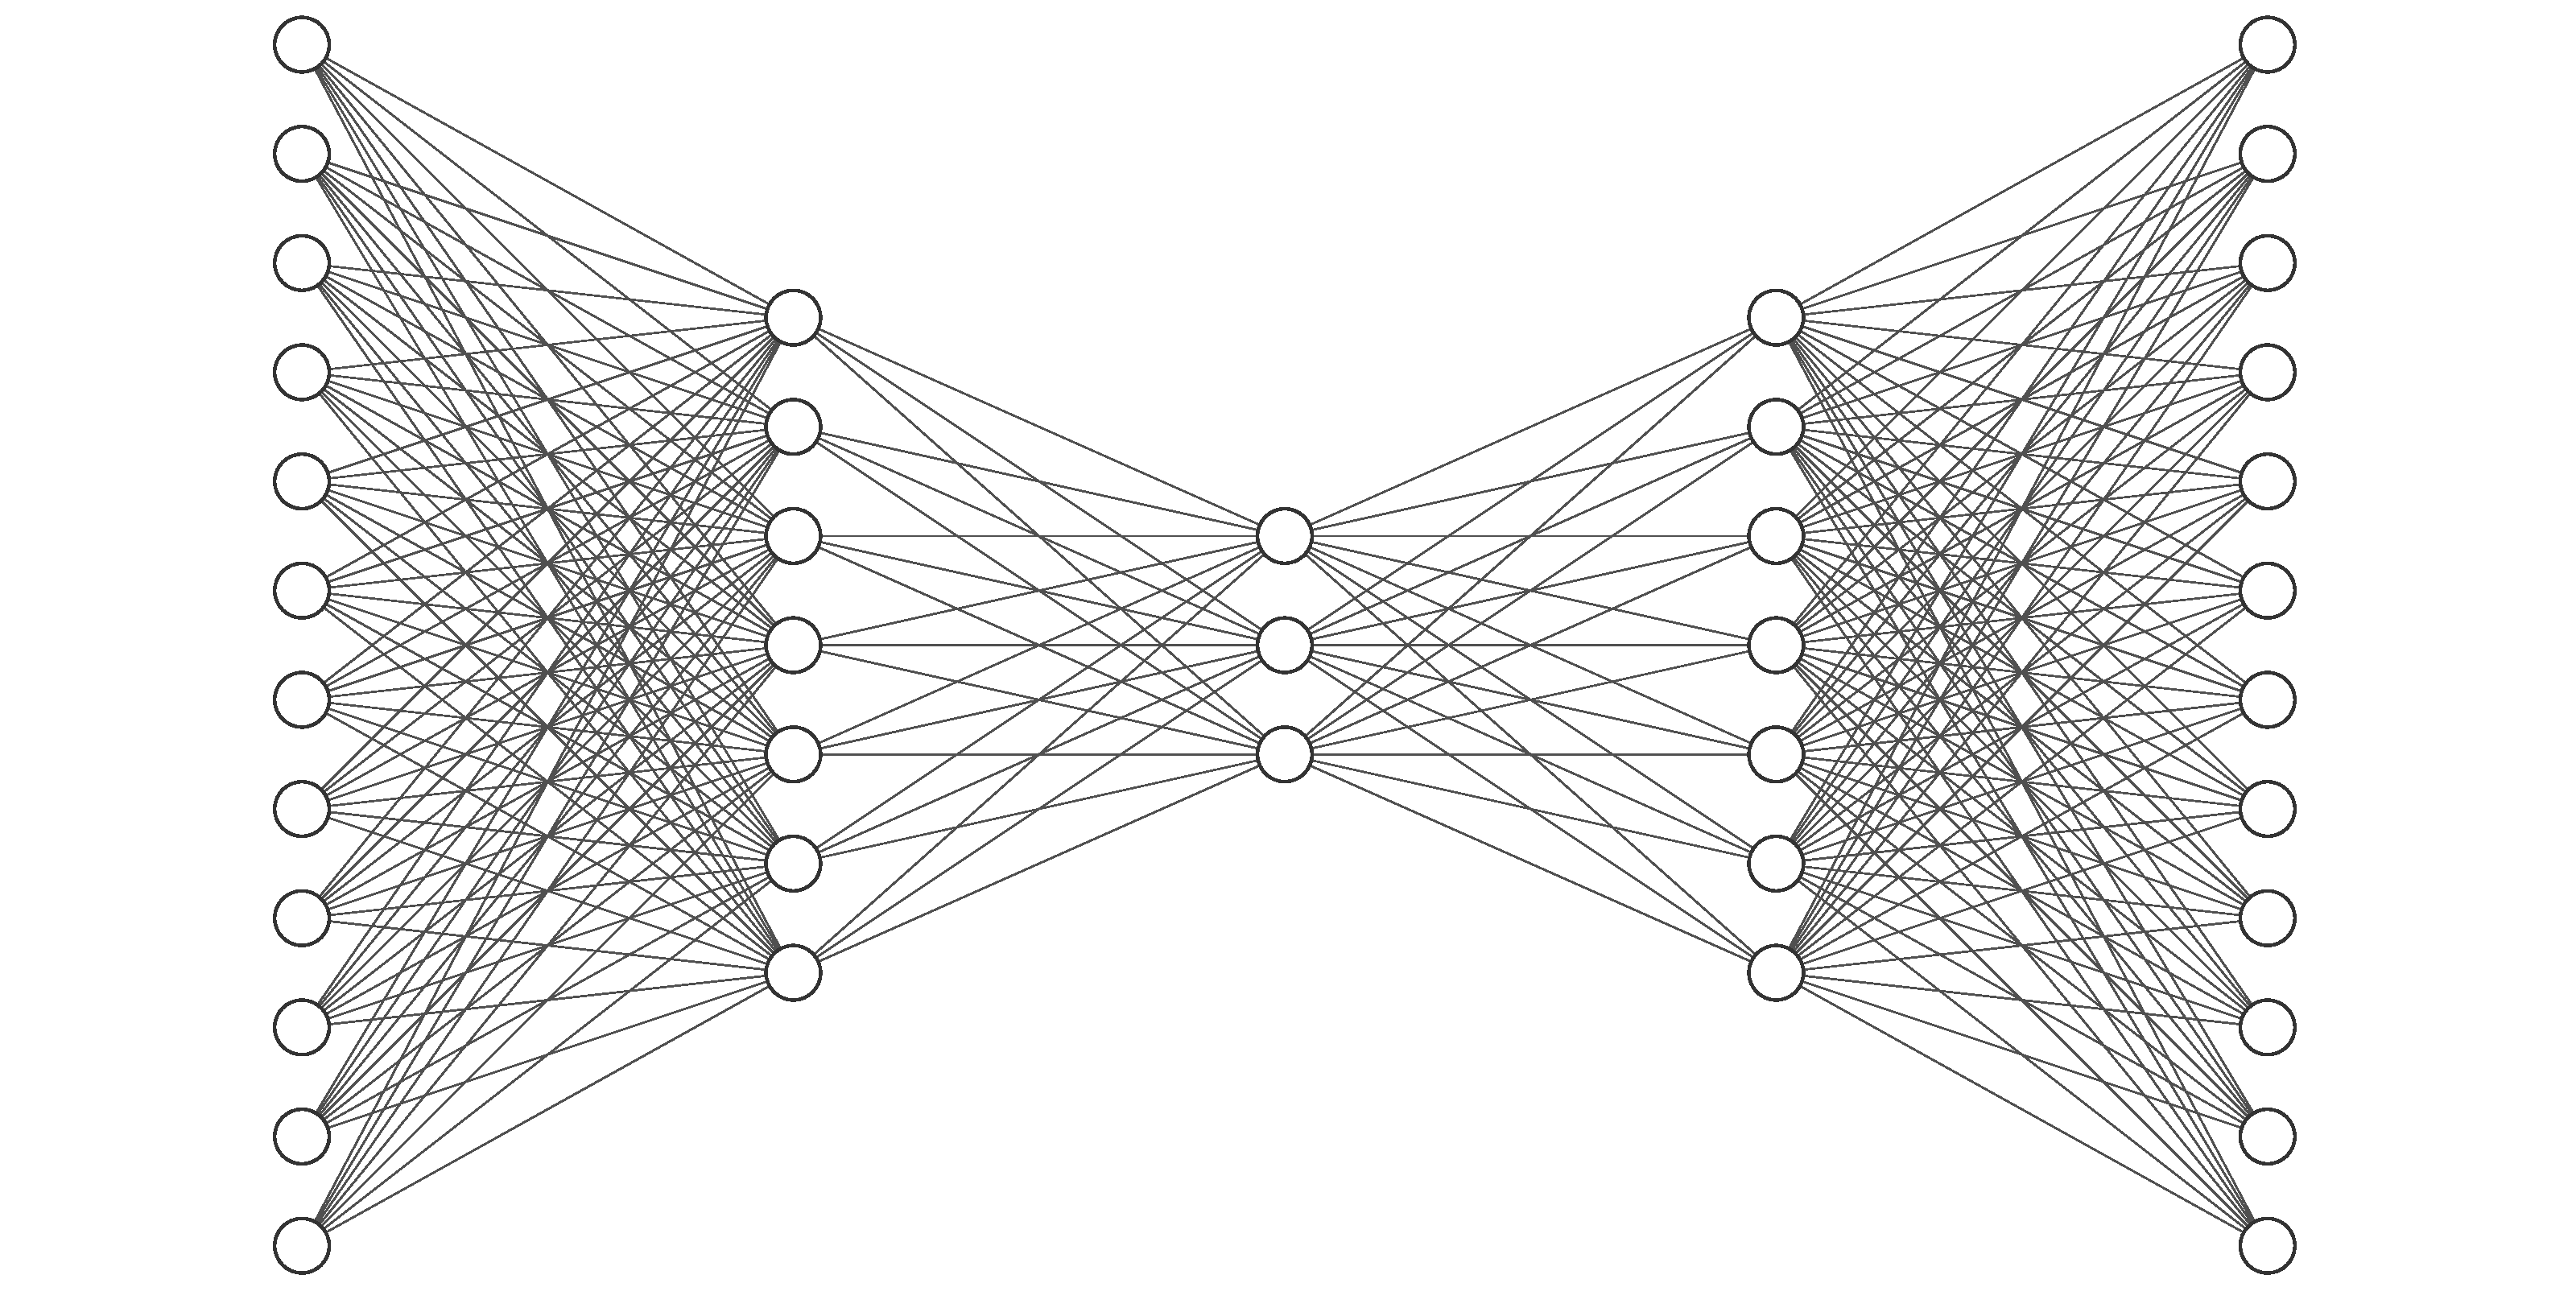
\includegraphics[width=\textwidth]{5_layer_AE.pdf}
		\caption[Schematische Abbildung der Architektur eines Autoencoders]{Gezeigt ist eine schematische Abbildung der Architektur eines (\textit{vollvernetzten}) Autoencoders. Dieser Autoencoder besitzt fünf Schichten, wobei das \textit{Bottleneck} dreidimensional und die \textit{Input}-Dimension zwölf ist. Das bedeutet, dass ein 12-dimensionaler Inputvektor in der Mitte des Autoencoders durch einen dreidimensionalen Vektor kodiert und anschließend wieder dekodiert werden muss, um zu einer möglichst verlustfreien Rekonstruktion zu gelangen. Eigene Darstellung, erstellt mittels \href{https://alexlenail.me/NN-SVG/}{NN-SVG}}
	\end{center}
\end{figure}

\subsubsection{Mathematische Formulierung}
\label{ch:MethodenDerDimRed:ML:AE:MathematischeFormulierung}
Mathematisch gesehen versucht der Autoencoder zwei Funktionen zu lernen. Zum einen den sogenannten \newterm{Encoder} $f: \real^D \rightarrow \real^d$, der den Inputvektor in die niedrigdimensionale Repräsentation $\rvect{y} = f(\rvect{x})$ codiert und zum anderen den \newterm{Decoder} $g: \real^d \rightarrow \real^D$, der diese Repräsentation wieder in den Inputvektor dekodiert. Das Ziel des Autoencoders ist es, den Inputvektor zu rekonstruieren und dabei eine sinnvolle Repräsentation im Bottleneck zu lernen:
\begin{equation}
	\estNormal{\rvect{x}} = g(f(\rvect{x})) \approx \rvect{x}
\end{equation}
wobei $\estNormal{\vect{x}}$ die Rekontruktion des Autoencoders bezeichnet.
Dazu minimiert der Autoencoder einen \newterm{Rekonstruktionsfehler} $L(\vect{x}, \vect{\estNormal{x}})$, der eine Ungleichheit zwischen dem Input- und Outputvektor bestraft. Hier wird meistens die quadratische Abweichung der beiden Vektoren verwendet, das heißt
\begin{equation}
	\label{eq:MSE_loss}
	L(\vect{x}, \vect{\estNormal{x}}) = L(\vect{x}, g(f(\vect{x}))) = \norm[\big]{\vect{x} - g(f(\vect{x}))}^2
\end{equation}
\parencite[507]{Goodfellow.2016}. Die Zielfunktion $\mathcal{J}_{\text{AE}}$, die der Autoencoder
minimiert, ist dann beispielsweise der Mittelwert über die Fehlerfunktion in den Trainingsdaten:
\begin{equation}
	\label{eq:AE_objectiveFunction}
	\mathcal{J}_{\text{AE}} = \frac{1}{n} \sum_{i = 1}^n L(\vect{x}_i, \estNormal{\vect{x}}_i)
\end{equation}
Eine weitere Möglichkeit ist der \newterm{Binary Cross-Entropy Loss}, wenn die Daten im Intervall $[0, 1]$ liegen.\unsure{wirklich das erwähnen?}

Die Gefahr dabei ist, dass der Autoencoder bei zu großer Kapazität einfach die Identitätsfunktion
ohne sinnvolle Repräsentation lernt. Dies ist zum Beispiel der Fall, wenn zu viele Schichten
eingesetzt werden und der Autoencoder einfach die Inputvektoren auf Indizes abbildet. Aus diesem
Grund muss ein Autoencoder oftmals regularisiert werden, worauf im Folgenden in
\subsecref{ch:MethodenDerDimRed:ML:AE:Regularisierung} eingegangen wird.

\subsubsection{Regularisierung}
\label{ch:MethodenDerDimRed:ML:AE:Regularisierung}
Um eine sinnvolle Repräsentation $\rvect{y}$ zu erhalten, muss der Autoencoder oftmals
regularisiert, das heißt eingeschränkt, werden. Ein erstes Beispiel hierfür ist der in
\figref{fig:5-layer-Autoencoder} gezeigte unterbestimmte Autoencoder, mit dem eine $d$-dimensionale
Repräsentation in der Mitte forciert wird. Besitzt der Autoencoder jedoch eine zu große Kapazität,
das heißt es werden zu viele Schichten eingesetzt, dann kann der Autoencoder trotz des Bottlenecks
eine uninformative niedrigdimensionale Repräsentation lernen, auch wenn das Bottleneck nur
eindimensional ist. Neben dieser \textit{impliziten} Regularisierung, gibt es deswegen noch einige
weitere \textit{explizite} Regularisierungsmethoden, die zusätzlich zum Rekonstruktionfehler einen
Bestrafungsterm $\Omega$ zur Fehlerfunktion $L$ hinzufügen. Die Zielfunktion lautet dann
\begin{equation}
	\mathcal{J}_{\text{AE+reg}} = \sum \left( L(\vect{x}, \estNormal{\vect{x}}) + \lambda \Omega \right)
\end{equation}
wobei $\lambda \geq 0$ ein \textit{Hyperparameter} ist, der die Stärke der Regularisierung kontrolliert. Damit muss der Autoencoder zwischen zwei entgegengesetzten Kräften balancieren: Einerseits muss der Autoencoder lernen, den Inputvektor zu rekonstruieren um den Rekonstruktionfehler gering zu halten. Andererseits darf der Bestrafungsterm nicht zu groß werden, was triviale Lösungen mit uninformativem Bottleneck ausschließen soll. Insgesamt wird sich dadurch also eine informativere niedrigdimensionale Repräsentation erhofft \parencite[516]{Goodfellow.2016}.

Eine Umsetzung dessen ist zum Beispiel der \newterm{Sparse Autoencoder}, der eine dünn besetzte
(engl. \textit{sparse}) Repräsentation $\vect{y}$ erzwingt, das heißt nur wenige Einträge von
$\vect{y}$ sind ungleich Null. Für das Lernen von Mannigfaltigkeiten besonders interessant ist
jedoch der \newterm{Contractive Autoencoder} \parencite{Rifai.2011}, der im \subsecref{ch:MethodenDerDimRed:ML:CAE} genauer behandelt wird. Wie
eingangs erwähnt ist ein linearer Autoencoder sehr ähnlich zur Hauptkomponentenanalyse. Dieser
Zusammenhang wird im Folgenden betrachtet.

\subsubsection{Verhältnis zur Hauptkomponentenanalyse}
\label{ch:MethodenDerDimRed:ML:AE:VerhaeltnisPCA}

\textcites{Baldi.1989}{Bourlard.1988} haben gezeigt, dass die Kodierung $\vect{y}$ eines linearen Autoencoders äquivalent -- aber nicht identisch -- zu den Hauptkomponenten einer PCA (siehe \secref{ch:MethodenDerDimRed:statistisch:PCA}) ist: Die Gewichte des Autoencoders spannen den gleichen Unterraum auf wie die Eigenvektoren der Kovarianzmatrix der Daten. Dies gilt sogar dann, wenn in einem dreischichtigen Autoencoder nichtlineare Aktivierungsfunktionen verwendet werden \parencite[291, 293]{Bourlard.1988}. Jedoch unterscheidet sich die Lösung eines linearen Autoencoders
mit der von PCA wie folgt \parencite[3]{Plaut.2018}:\unsure{was meine ich mit "Lösung" des linearen Autoencoders? Genauer
	beschreiben}
\begin{enumerate}
	\item Die Lösung eines linearen Autoencoders ist nicht orthogonal, das heißt sie ist nicht unkorrelliert.
	\item Die Lösung eines linearen Autoencoders ist nicht absteigend nach zugehöriger Varianz sortiert.
	\item Die Lösung einer Reduktion auf $k_1$ Neuronen in der Bottleneck-Schicht ist keine Teilmenge für
	      eine Reduktion auf $k_2$ Neuronen mit $k_2 < k_1$.
\end{enumerate}
%Um den Zusammenhang zwischen der PCA und dem Autoencoder zu verdeutlichen,
% wird im Folgenden ein einfacher linearer Autoencoder mit drei Schichten betrachtet. Der Encoder
% kann somit als
% \begin{equation}
% 	f(\vect{x}) = \mat{W}_1 \vect{x} + \vect{b}_1 = \vect{y}
% \end{equation}
% und der Decoder als
% \begin{equation}
% 	g(\vect{y}) = \mat{W}_2 \vect{y} + \vect{b}_2 = \estNormal{\vect{x}}
% \end{equation}
% formuliert werden, wobei $\mat{W}_1 \in \real^{d \times D}$ und $\mat{W}_2 \in \real^{D \times d}$ die Gewichtsmatrizen und $\vect{b}_i$ die Bias-Vektoren des Autoencoders sind ($i = 1, 2$). Liegt eine Stichprobe in der Datenmatrix $\mat{X} \in \real^{n \times D}$ vor und minimiert der Autoencoder den mittleren quadratischen Fehler (\eqref{eq:MSE_loss}), dann löst dies\rewrite{das ganze hier bringt mir irgendwie nichts}
% \begin{equation}
% 	\min \norm{ \mat{X} - \tr{ \left( \mat{W}_2( \mat{W}_1 \tr{\mat{X}} + \vect{b}_1 \tr{\ones_n}) + \vect{b}_2 \tr{\ones_n}  \right) } }^2_F
% \end{equation}\rewrite{oben die Gewichtsmatrizen transponieren, dann muss ich nicht die Daten transponieren}
% wobei $\ones_D = \tr{(1, \ldots, 1)} \in \real^D$ der Vektor mit Einsen und $\norm{\,\cdot\,}_F$ die Frobenius-Norm ist \parencite[3]{Plaut.2018}.
\subsection{Contractive Autoencoder}
\label{ch:MethodenDerDimRed:ML:CAE}
\nomenclature[Z]{CAE}{Contractive Autoencoder}

Der Contractive Autoencoder \parencite{Rifai.2011} stellt eine Variante des eben vorgestellten klassichen Autoencoders
\subsecref{ch:MethodenDerDimRed:ML:AE} dar. Ähnlich wie der Sparse Autoencoder wird die
Zielfunktion des Autoencoders lediglich um einen zusätzlichen Regularisierungsterm erweitert. Dies
führt zu einer kontrahierenden Eigenschaft: Ähnliche Punkte werden auf eine kleinere
Nachbarschaften auf der Mannigfaltigkeit abgebildet und damit \enquote{zusammengezogen}. Dies gilt
aber nur \textit{lokal}, das heißt unähnliche Punkte können immer noch weit weg auf der
Mannigfaltigkeit liegen \parencite[521]{Goodfellow.2016}. Dazu wird wieder in \subsecref{ch:MethodenDerDimRed:CAE:Grundidee}
auf die Grundidee eingegangen und dann in \subsecref{ch:MethodenDerDimRed:ML:CAE:BerechnungRegTerm}
die konkrete Berechnung des Regularisierungsterms vorgestellt.

\subsubsection{Grundidee}
\label{ch:MethodenDerDimRed:CAE:Grundidee}
Die Idee ist
es, die \textit{Sensitivität} des Autoencoders für den Input zu bestrafen. Das bedeutet, dass bei
kleinen Änderungen des Inputs $\vect{x}$ die Kodierung $f(\vect{x})$ ebenfalls nur minimal geändert
werden soll. Dies entspricht einer kleinen ersten Ableitung und kann über die (quadrierte)
Frobeniusnorm der Jacobi-Matrix $\mat{J}$ des Encoders $f$ erzielt werden \parencites[2]{Rifai.2011}[521]{Goodfellow.2016}. Der Regularisierungsterm lautet damit
\begin{equation}
	\label{eq:CAE-Regularisierung}
	\Omega(\vect{y}) = \norm[\big]{\mat{J}_f(\vect{x})}_F^2 =  \norm[\Big]{ \frac{\partial f(\vect{x})}{\partial \vect{x}} }^2_F
\end{equation}
was der Summe über die quadrierten Einträge der Jacobi-Matrix entspricht. Intuitiv gesehen werden so lokale Nachbarschaften auf \textit{kleinere} Nachbarschaften in der niedrigdimensionalen Repräsentation abgebildet, das heißt der Autoencoder wirkt kontrahierend.
Der Regularisierungsterm ist, wie wir in \subsecref{ch:MethodenDerDimRed:ML:CAE:BerechnungRegTerm} sehen werden, für einen dreischichtigen Autoencoder leicht zu berechnen, nicht aber für einen tiefen Autoencoder. Dies stellt ein praktisches Problem dar, welches allerdings über ein schichtenweises vortrainieren teilweise umgangen werden werden kann \parencite[vgl.][522]{Goodfellow.2016}.

\subsubsection{Berechnung des Regularisierungsterms}
\label{ch:MethodenDerDimRed:ML:CAE:BerechnungRegTerm}
Der Regularisierungsterm ist wie eben erwähnt für einen Autoencoder mit nur einer versteckten Schicht leicht zu berechen. Der Encoder
kann in diesem Fall als
\begin{equation}
	f(\vect{x}) = s \left( \mat{W} \vect{x} + \vect{b}_1 \right) = \vect{y}
\end{equation}
und der Decoder als
\begin{equation}
	g(\vect{y}) = s \left( \mat{\widetilde{W}} \vect{y} + \vect{b}_2 \right) = \estNormal{\vect{x}}
\end{equation}
formuliert werden, wobei $\mat{W} \in \real^{d \times D}$ und $\mat{\widetilde{W}} \in \real^{D \times d}$ die Gewichtsmatrizen und $\vect{b}_i$ die Bias-Vektoren des Autoencoders sind ($i = 1, 2$). Dies entspricht jeweils einer affinen Transformation gefolgt von einer (nichtlinearen) Aktivierungsfunktion. Gilt außerdem, dass die Gewichte des Encoders und Decoders verbunden sind, das heißt $\mat{\widetilde{W}} = \tr{\mat{W}}$ und wird für die Aktivierungfunkion $s$ die Sigmoid-Funktion
\begin{equation}
	\operatorname{sigmoid}(\vect{x}) = \frac{1}{1 + \exp (-\vect{x})}
\end{equation}
verwendet, so kann die Frobeniusnorm der Jacobi-Matrix mittels
\begin{equation}
	\norm[\big]{\mat{J}_f(\vect{x})}_F^2 = \sum_{i = 1}^d \left( \vect{y}_i (1 - \vect{y}_i)\right)^2 \sum_{ij} \mat{W}^2_{ij}
\end{equation}\unsure{was sind hier die Grenzen der Summen ? n oder d, D?}
effizient berechnet werden \parencite[4]{Rifai.2011}. Für einen Autoencoder mit mehr als einer versteckten Schicht gibt es keine
geschlossene Form mehr und die Berechnung wird teuer, was das Trainieren eines tiefen Contractive
Autoencoders ohne Tricks wie beispielsweise das gierige schichtenweise vortrainieren (engl.
\textit{greedy layerwise pre-training}) unpraktikabel macht. Bei diesem Vorgehen wird ein tiefer
Autoencoder schichtenweise durch untiefe Autoencoder (drei Schichten) vortrainiert und im letzten
Schritt erfolgt eine Feinabstimmung des kompletten Netzwerks (engl. \textit{fine-tuning}) \parencite[522]{Goodfellow.2016}. Dieses Vorgehen kann analog auch für klassische Autoencoder verwendet
werden, um eine gute Initialisierung der Gewichte zu erreichen und damit suboptimale lokale Minima
der Zielfunktion zu umgehen \parencite[509]{Goodfellow.2016}.